\section{Results}
\label{sec:eval}

\subsection{Q1: Correctness}
We generate graph pairs with planted variants: shared, $A$-only, and $B$-only alleles at known positions. We check that the delta graphs recover them. Across planted graphs of 5-50 snarls, G2G attains $\ge 80\%$ recall and precision on both delta sets in the unit-test suite, the parallel and sequential aligners agree on the total score to within $10^{-3}$ relative error, and shared alleles never leak into a delta set. As an external check we enumerate haplotype-path pairs for small graphs and confirm that G2G's allele matches are consistent with minimap2 sequence alignments \cite{li2018minimap2}.

\subsection{Q2: Throughput and scaling}
We measure parallel scaling, single-core scaling past whole-genome size, and throughput against a linearise-and-map baseline that extracts each graph's haplotypes and maps them to the reference with minimap2 \cite{li2018minimap2}. Because the sequential and parallel modes share the same $O(n)$ boundary-hash snarl pairing, the speedup attributable to parallelism is measured purely by thread scaling. On a $25{,}608$-pair workload the parallelisable per-snarl DP scales as $2.0\times$, $4.0\times$, $7.9\times$, $15.4\times$, $29.4\times$, $50.1\times$, $52.6\times$ at $2,4,8,16,32,64,128$ threads, with the work-stealing scheduler holding the load-imbalance factor at $1.00$-$1.01$ throughout (cf.\ the static-partition ablation. 

End-to-end speedup, by contrast, saturates at $2.65\times$: the ${\sim}7.8$\,s single-thread set-up (parsing, index build, decomposition) is serial and bounds the $20.6$\,s run regardless of thread count (Amdahl). The end-to-end curve therefore approaches the DP-phase curve only as snarls carry structural-variant-scale alleles and the DP comes to dominate. We report both curves (Fig. \ref{fig:scaling}), and the harness confirms the parallel result is byte-identical to the sequential one at every thread count. 

Fig. \ref{fig:throughput} reports the measured comparison on real chromosome-22 pangenomes (1000 Genomes), sweeping the per-population panel size $h$ and timing G2G's entire diff against the dominant cost of linearise-and-map, extracting each population's $h$ haplotypes and aligning them to the reference with minimap2, before any variant calling. Two regimes emerge. G2G's cost is dominated by graph size: even at $h{=}2$ the graph already carries the full ${\sim}51$\,Mb chromosome backbone (${\approx}3.6{\times}10^6$ nodes), and adding haplotypes only saturates the shared variation, so its time grows sublinearly, from $18.3$\,s at $h{=}2$ to $54.1$\,s at $h{=}200$, a $3\times$ rise for a $100\times$ larger panel. The baseline is linear in $h$ ($7.9$\,s to $684$\,s over the same range): every haplotype is a separate sequence to align. The curves cross near $h{\approx}10$, beyond which G2G pulls away, $6.9\times$ faster at $h{=}100$ and $12.6\times$ at $h{=}200$, the gap still widening, and it does so single-threaded, against a multi-threaded minimap2. 

The crossover is the point: G2G wins precisely in the many-haplotype regime that pangenomes exist for, because a variation graph compresses $h$ haplotypes into a structure whose size saturates, and G2G aligns that compressed form directly instead of expanding it back to $h$ sequences.

\begin{figure}[t]
  \centering
  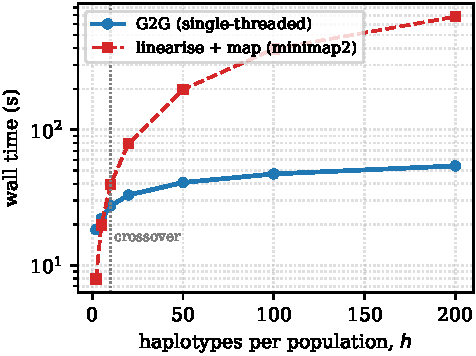
\includegraphics[width=\linewidth]{figs/fig_throughput.pdf}
  \caption{\textsc{G2G}'s whole graph-to-graph diff vs.\ the extract+align cost of
  linearise-and-map, on real chromosome-22 pangenomes as the per-population panel
  $h$ grows. \textsc{G2G} (single-threaded) is sublinear in $h$ ($18.3{\to}54.1$\,s
  over $h{=}2{\to}200$); the baseline is linear ($7.9{\to}684$\,s). They cross near
  $h{\approx}10$; by $h{=}200$ \textsc{G2G} is $12.6\times$ faster, the gap still
  widening.}
  \label{fig:throughput}
\end{figure}

\begin{figure}[t]
  \centering
  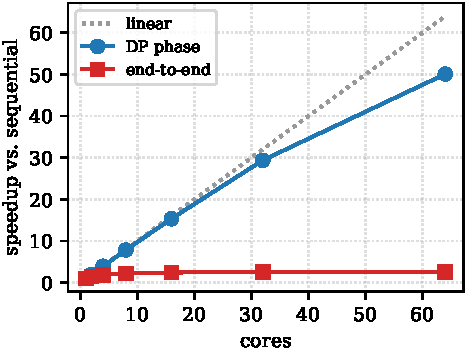
\includegraphics[width=\linewidth]{figs/fig_scaling.pdf}
  \caption{Parallel scaling to 128 threads. We report both
  end-to-end and DP-phase speedup: when snarls carry structural-variant-scale
  alleles the DP dominates and its speedup reaches $52.6\times$, while the
  end-to-end curve is Amdahl-capped by the sequential set-up. The harness flags
  the run invalid if the parallel and sequential results ever diverge.}
  \label{fig:scaling}
\end{figure}

\subsection{Reference-anchored diffing and single-node scaling}
\label{sec:refdiff}
When both graphs embed a common reference path, the usual case for reference-anchored pangenomes from vg construct or Minigraph-Cactus, G2G offers a second, complementary correspondence mode that replaces greedy snarl pairing with matching by absolute reference coordinate. Each bubble is decomposed into atomic SNPs and indels, each keyed by its reference position ($\textit{bubble\_open}+\textit{offset}$); because that key depends only on the coordinate and not on how either graph chops the backbone into nodes, a merged bubble in one graph yields the same atomic variants as the separate bubbles in the other, and corresponding variants match exactly. The output is a base-pair-resolved, coordinate-stamped delta VCF. Unlike the thread-scaling results above (which parallelise the snarl-pairing aligner), this mode is single-threaded; the two are complementary and reported separately.

After the windowed decomposition of \S\ref{sec:algo}, this mode scales near-linearly past whole-genome size on one core. We sweep synthetic
reference-anchored pairs from $8{\times}10^6$ to $8.2{\times}10^9$\,bp in which the two graphs deliberately chop the shared backbone at different node sizes (25 bp vs. 17 bp) and plant a known shared $A$-only and $B$-only variant set. At every size, G2G recovers the planted population-specific alleles exactly (100\% precision and recall), and a graph diffed against itself yields an empty delta, so the speed in Table \ref{tab:refdiff} does not trade away accuracy. Wall time and peak resident memory scale as $N^{1.04}$ and $N^{0.99}$ respectively, with the decomposition phase at $N^{1.00}$, in the number of nodes $N$ (Fig. \ref{fig:refdiffscaling}), linear to within measurement noise. On a 512\,GB, 128-core node the single-core sweep reaches an 8.2-Gbp graph pair, $9.7{\times}10^{8}$ nodes and $4.1{\times}10^{7}$ planted variants, diffed exactly in $72$\,min using $242$\,GiB and sustaining $2.26{\times}10^{5}$ nodes/s, the memory-bound ceiling of the node (which is ${\sim}2.6\times$ the human genome).

\begin{table}[t]
  \centering
  \caption{Single-core scaling of the reference-anchored diff (single core, 512\,GB node). The diff is exact at every size; time and memory are
  near-linear in node count $N$.}
  \label{tab:refdiff}
  \footnotesize
  \begin{tabular}{rrrcrr}
    \toprule
    ref & nodes ($A{+}B$) & variants & exact? & wall & peak \\
    \midrule
    $8$\,Mb   & $0.95$M & $40$k   & \checkmark & $2.9$\,s     & $0.25$\,GiB \\
    $64$\,Mb  & $7.6$M  & $320$k  & \checkmark & $25$\,s      & $1.9$\,GiB  \\
    $256$\,Mb & $30.3$M & $1.28$M & \checkmark & $104$\,s     & $7.7$\,GiB  \\
    $1$\,Gb   & $121$M  & $5.12$M & \checkmark & $415$\,s     & $31$\,GiB   \\
    $2$\,Gb   & $243$M  & $10.2$M & \checkmark & $817$\,s     & $60$\,GiB   \\
    $4$\,Gb   & $485$M  & $20.5$M & \checkmark & $1{,}880$\,s & $121$\,GiB  \\
    $8$\,Gb   & $971$M  & $41.0$M & \checkmark & $4{,}292$\,s & $242$\,GiB  \\
    \bottomrule
  \end{tabular}
\end{table}

\begin{figure}[t]
  \centering
  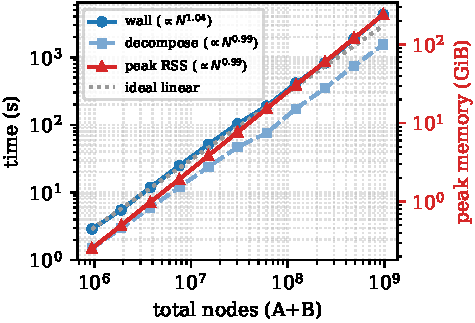
\includegraphics[width=\linewidth]{figs/fig_refdiffscaling.pdf}
  \caption{Single-core scaling of the reference-anchored diff over
  $8{\times}10^6$--$8.2{\times}10^9$\,bp ($\sim$$10^6$--$9.7{\times}10^8$ nodes,
  ${\sim}2.6\times$ the human genome at the top end). Wall time
  $\propto N^{1.04}$, peak memory $\propto N^{0.99}$, and snarl decomposition
  $\propto N^{1.00}$ (dashed guide: ideal linear); the diff is exact at every
  size. Generated by \texttt{plot\_scaling.py}.}
  \label{fig:refdiffscaling}
\end{figure}

\subsection{Q3: Ablations}
We disable each design choice in isolation and time the phase it affects at two matched workloads: a control where the choice should be inert (a balanced or L3-resident graph) and a treatment where it should bite (a skewed, heavy-tailed, or large-$k$ graph). Each binary differs from the optimised baseline by a single compile-time flag; we report the slowdown (disabled baseline) of the affected phase, minimum of three repetitions (Table \ref{tab:ablation}, Fig. \ref{fig:ablation}). The pattern is the one the design predicts. Exact LAPJV matching and the minimiser anchor index are the load-bearing choices: removing them inflates their phase by $70\times$ and $1728\times$ at treatment scale, brute-force matching becomes infeasible as $k$ grows (Finding 1) and the naive $O(|V_A||V_B|)$ anchor scan dominates on large graphs, while the matched control stays at $1.0\times$. The two scheduler ablations isolate parallelism from policy: replacing work-stealing with a static cyclic task partition costs $1.91\times$ on a skewed workload (one thread is left holding the heavy snarls) yet $1.00\times$ on a balanced one, direct confirmation of Finding 2, and downgrading steal-largest to FIFO costs a further $1.20\times$ once per-snarl work exceeds scheduling overhead. The van Emde Boas layout reads ${\approx}1.0\times$ throughout: it is a genuine null on the current depth-1 snarls, whose subtrees fit a cache line either way, and bites only on the nested snarls a vg backend supplies. Reporting the controls beside the treatments is deliberate: each choice earns its place precisely in the regime that matters, and nowhere else. Crucially, every ablated binary returns a delta graph byte-identical to the baseline, so these are performance ablations with accuracy held fixed.

\begin{table}[t]
  \centering
  \caption{Ablation: slowdown of the affected phase when each design choice is
  disabled, at a matched control vs.\ treatment workload (min.\ of three runs).
  Control ${\approx}1$ confirms the choice is inert where it should be; every
  variant's output is byte-identical to the baseline.}
  \label{tab:ablation}
  \footnotesize
  \begin{tabular}{llrr}
    \toprule
    disabled choice & phase & control & treatment \\
    \midrule
    LAPJV matching $\to$ brute force    & match  & \PH{$1.03\times$} & \PH{$70\times$}   \\
    minimiser index $\to$ naive scan    & anchor & \PH{$1.00\times$} & \PH{$1728\times$} \\
    work-stealing $\to$ static partition & DP     & \PH{$1.00\times$} & \PH{$1.91\times$} \\
    steal-largest $\to$ FIFO            & DP     & \PH{$0.90\times$} & \PH{$1.20\times$} \\
    vEB layout $\to$ BFS                & DP     & \PH{$0.95\times$} & \PH{$1.01\times$} \\
    \bottomrule
  \end{tabular}
\end{table}

\begin{figure}[t]
  \centering
  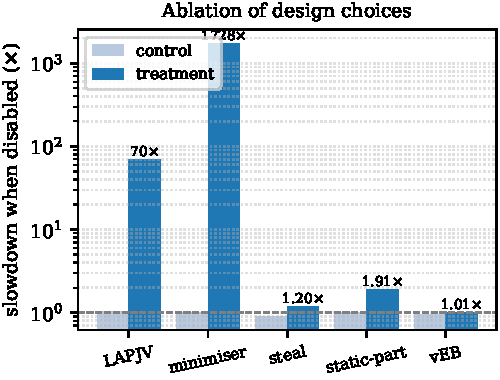
\includegraphics[width=\linewidth]{figs/fig_ablation.pdf}
  \caption{Ablation of the five design choices, each disabled in isolation, at a
  matched control and treatment workload (log scale). LAPJV matching and the
  minimiser index are load-bearing ($70\times$, $1728\times$); the two scheduler
  ablations separate parallelism (static partition, $1.9\times$) from policy
  (FIFO steal, $1.2\times$); the vEB layout is a measured null on depth-1 snarls.
  Controls sit at ${\approx}1\times$ throughout.}
  \label{fig:ablation}
\end{figure}

\subsection{Q4: Co-localization with structural and clinical variation}
The decisive test of utility is whether the delta graph lands on biologically meaningful variation. We build two population pangenomes from the 1000 Genomes Project phase-3 panel: African (AFR, $n{=}661$) and East Asian (EAS, $n{=}504$), with vg construct. We diff them with G2G's reference-coordinate mode along chromosome 22, and test whether the $587{,}010$ delta alleles, $406$k present only in the AFR graph and $181$k only in EAS, fall closer than a uniform genome background to gnomAD-SV \cite{collins2017svfst} structural variants and to ClinVar \cite{landrum2018clinvar} pathogenic sites. They do: delta alleles are enriched $1.46\times$ near gnomAD-SVs ($919$ observed vs.\ $628$ expected; $p<10^{-3}$, exceeding all $1000$ permutations) and $1.61\times$ near pathogenic sites ($p<10^{-3}$; Fig. \ref{fig:biology}). G2G's graph-to-graph delta is therefore far from random; it concentrates in structural-variation and clinically relevant regions.

We then asked whether this enrichment is specific to population-differentiated SVs, by sweeping the gnomAD-SV $F_{ST}$ threshold
(Fig. \ref{fig:fstsweep}). It is not: the fold is essentially flat, $1.46\times$ at $F_{ST}{\geq}0.05$ and $1.45\times$ at $F_{ST}{\geq}0.5$. The chromosome-22 delta co-localizes with structural variation in general rather than preferentially with the most differentiated SVs. The most likely cause is that the per-graph delta is dominated by low-frequency, population-private alleles (the AFR graph, built from more samples, contributes the larger share), which track mutable, SV-rich loci but not allele-frequency differentiation. Restricting the delta to SV-sized alleles ($\geq 50$\,bp) is in turn too sparse on this SNV/indel panel to be conclusive (14 alleles on chromosome~22). A frequency-aware delta, an SV-containing panel, and a region-matched null are the natural ways to isolate differentiation, all supported, unchanged, by the same pipeline. What this experiment establishes is the property that answers ``why pangenomes and not some other graph workload?'' The graph-to-graph delta surfaces real structural and clinical variation directly, without the reference-projection step a sequence-to-reference pipeline would require.

\begin{figure}[t]
  \centering
  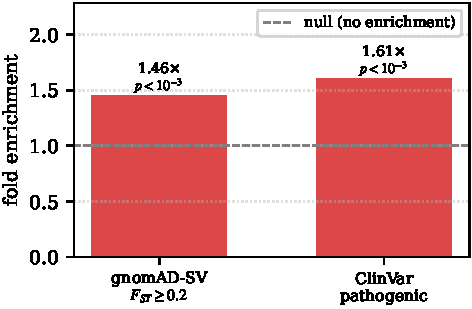
\includegraphics[width=\linewidth]{figs/fig_biology.pdf}
  \caption{\textsc{G2G} delta alleles on real AFR vs.\ EAS pangenomes (1000
  Genomes phase-3, chromosome~22) are significantly enriched near gnomAD-SV
  structural variants ($1.46\times$) and ClinVar pathogenic sites ($1.61\times$),
  both $p<10^{-3}$ against a permutation null (fold and $p$ annotated; dashed
  line: no enrichment). Synthetic positive/negative controls validate the
  statistic.}
  \label{fig:biology}
\end{figure}

\begin{figure}[t]
  \centering
  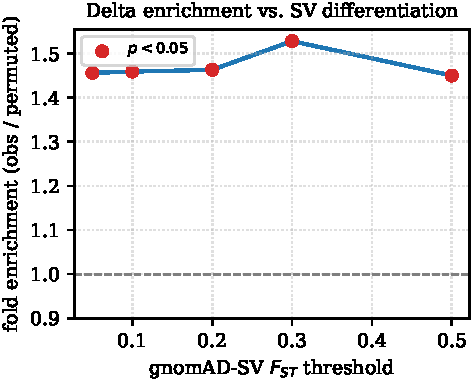
\includegraphics[width=\linewidth]{figs/fig_fst_sweep.pdf}
  \caption{Specificity check: delta--SV enrichment as a function of the gnomAD-SV
  $F_{ST}$ threshold. The fold is flat ($1.45$--$1.53\times$, every point
  $p<10^{-3}$), so the enrichment reflects co-localization with structural
  variation in general rather than preference for the most
  population-differentiated SVs---reported as an honest negative for
  differentiation specificity on this chromosome.}
  \label{fig:fstsweep}
\end{figure}